\section{Durchführung}
\subsection{Aufbau}
\begin{figure} [h]
    \centering
    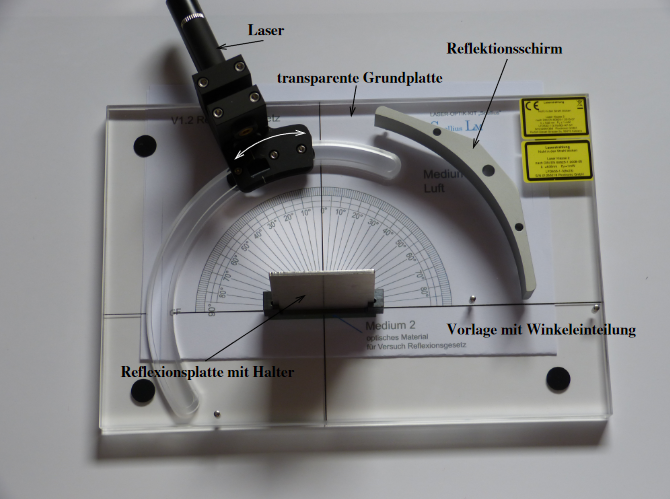
\includegraphics[width=12cm, keepaspectratio]{Reflexion Aufbau}
    \label{fig:Versuchsanordnung (Reflexion)}
    \caption{Reflexion}
 \end{figure}
Für diesen Versuch wird im wesentlichen eine transparente Glasplatte verwendet, auf der sich ein Modul mit regelbarem Winkel und zwei Laserdioden sowie ein Schirm befindet. Weiterhin existieren mehrere Unterlagen für die Platte, durch die Beispielsweise Anstell- oder Brechungswinkel abgelesen werden können. Der obere der beiden Laser emmitiert rotes Licht der Wellenlänge  $\lambda=635$ nm, der untere grünes Licht der Wellenlänge $\lambda=532$ nm. Außerdem können auf der Platte unterschiedliche optische Elemente platziert werden.
\subsection{Reflektion}
Für die erste Messreihe wird wie in Abbildung \ref{fig:Reflexion} ein Reflektor auf der Platte platziert. Anschließend wird für sieben unterschiedliche Einfallswinkel des Lasers der Ausfallswinkel gemessen.
\subsection{Brechung an den Platten}
Um die Brechung zu untersuchen wird der Laser auf eine planparallele Platte gerichtet. Auf dieser kann für sieben unterschiedliche Anstellwinkel an einer dafür an der Platte vorgesehenen Skala der Brechungswinkel abgelesen werden.\\
Wenn das Licht aus den Platten austritt kann ein Versatz $s$ des Lichtstrahls gegenüber dem ursprünglichen Strahl beobachtet werden, wie in Abbildung () gezeigt. Dieser kann aus den Einfalls- und Brechungswinkel gemäß
\begin{equation}
s=d \frac{\sin(\alpha - \beta)}{\cos(\beta)}
\end{equation}
mit der Plattendicke $d$ berechnet werden. \\
  \begin{figure} [h]
    \centering
    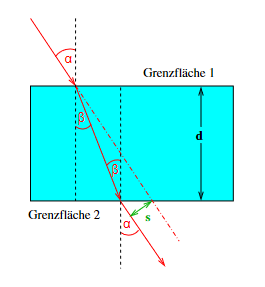
\includegraphics[width=6cm, keepaspectratio]{Planparallele Platten}
    \label{fig:Versatz}
    \caption{Geometrie der Lichtbrechung und Strahlenversatz}
 \end{figure}
\subsection{Brechung am Prisma}
Für diesen Versuch wird das Lasermodul auf ein Prisma gerichtet. Mithilfe der dafür vorgesehenen Unterlage kann wiederum für sieben verschiedene Anstellwinkel der Austrittswinkel bestimmt werden. Da die Laser sich in ihrer Wellenlänge unterscheiden, werden sie unterschiedlich stark gebrochen, sodass sich die Austrittswinkel unterscheiden.
Die Ablenkung $\delta$ kann durch
\begin{equation}
\delta=(\alpha_1 + \alpha_2)-(\beta_1 + \beta_2)
\end{equation}
\begin{figure} [h]
    \centering
    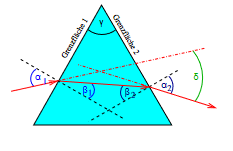
\includegraphics[width=6cm, keepaspectratio]{Brechung am Prisma}
    \label{fig:Prisma}
    \caption{Brechung am Prisma}
 \end{figure}
berechnet werden. Die Winkel $\beta_1$ bzw. $\beta_2$ werden dabei durch das Brechungsgesetz sowie den Zusammenhang $\beta_1+\beta_2=\gamma=60°$ bestimmt.
\subsection{Beugung}
Für den letzten Versuchsteil werden die Laser senkrecht auf ein Gitter gerichtet. Anschließend kann auf dem dafür vorgesehenen Schirm abgelesen werden, bei welchen Winkeln die Maxima liegen. Dieses Vorgehen wird für beide Laser an drei verschiedenen Gittern wiederholt. 
